\documentclass[12pt, a4paper]{article}
\usepackage{ctex}

\usepackage[margin=1in]{geometry}
\usepackage{
  color,
  clrscode,
  amssymb,
  ntheorem,
  amsmath,
  listings,
  fontspec,
  xcolor,
  supertabular,
  multirow,
  mathtools,
  mathrsfs
}
\definecolor{bgGray}{RGB}{36, 36, 36}
\usepackage[
  colorlinks,
  linkcolor=bgGray,
  anchorcolor=blue,
  citecolor=green
]{hyperref}
\newfontfamily\courier{Courier}

\theoremstyle{margin}
\theorembodyfont{\normalfont}
\newtheorem{thm}{定理}
\newtheorem{cor}[thm]{推论}
\newtheorem{pos}[thm]{命题}
\newtheorem{lemma}[thm]{引理}
\newtheorem{defi}[thm]{定义}
\newtheorem{std}[thm]{标准}
\newtheorem{imp}[thm]{实现}
\newtheorem{alg}[thm]{算法}
\newtheorem{exa}[thm]{例}
\newtheorem{prob}[thm]{问题}
\DeclareMathOperator{\sft}{E}
\DeclareMathOperator{\idt}{I}
\DeclareMathOperator{\spn}{span}
\DeclareMathOperator*{\agm}{arg\,min}
\newcommand{\pr}{\prime}
\newcommand{\tr}{^\intercal}
\newcommand{\st}{\text{s.t.}}
\newcommand{\hp}{^\prime}
\newcommand{\ms}{\mathscr}
\newcommand{\mn}{\mathnormal}
\newcommand{\tbf}{\textbf}
\newcommand{\mbf}{\mathbf}
\newcommand{\fl}{\mathnormal{fl}}
\newcommand{\f}{\mathnormal{f}}
\newcommand{\g}{\mathnormal{g}}
\newcommand{\R}{\mathbf{R}}
\newcommand{\Q}{\mathbf{Q}}
\newcommand{\JD}{\textbf{D}}
\newcommand{\rd}{\mathrm{d}}
\newcommand{\str}{^*}
\newcommand{\vep}{\varepsilon}
\newcommand{\lhs}{\text{L.H.S}}
\newcommand{\rhs}{\text{R.H.S}}
\newcommand{\con}{\text{Const}}
\newcommand{\oneton}{1,\,2,\,\dots,\,n}
\newcommand{\aoneton}{a_1a_2\dots a_n}
\newcommand{\xoneton}{x_1,\,x_2,\,\dots,\,x_n}
\newcommand\thmref[1]{定理~\ref{#1}}
\newcommand\lemmaref[1]{引理~\ref{#1}}
\newcommand\defref[1]{定义~\ref{#1}}
\newcommand\posref[1]{命题~\ref{#1}}
\newcommand\secref[1]{节~\ref{#1}}
\newcommand\equref[1]{(\ref{#1})}
\newcommand\figref[1]{图 \ref{#1}}
\newcommand\corref[1]{推论~\ref{#1}}
\newcommand\exaref[1]{例~\ref{#1}}
\newcommand\algref[1]{算法~\ref{#1}}
\newcommand{\remark}{\paragraph{评注}}
\newcommand{\example}{\paragraph{例}}
\newcommand{\proof}{\paragraph{证明}}


\title{E06c 编程作业解答}
\author{姓名:任云玮$\quad$学号:516030910586}
\date{}

\usepackage{titlesec}

\titleformat*{\section}{\large\bfseries}
\titleformat*{\subsection}{\normalsize\bfseries}
\newcommand{\ilc}{\texttt}

\begin{document}
\lstset{
  numbers=left,
  basicstyle=\scriptsize,
  numberstyle=\tiny\color{red!89!green!36!blue!36},
  language=Matlab,
  breaklines=true,
  keywordstyle=\color{blue!70},commentstyle=\color{red!50!green!50!blue!50},
  morekeywords={},
  stringstyle=\color{purple},
  frame=shadowbox,
  rulesepcolor=\color{red!20!green!20!blue!20}
}
\maketitle

\paragraph{问题}
  用不同数值方法计算积分
  \[
    \int_0^1\sqrt{x}\ln x\rd x = -\frac{4}{9}.
  \]

\section{复化求积方法}
\subsection{图像及作图相关代码}
  \begin{figure}[htbp]
    \centering
    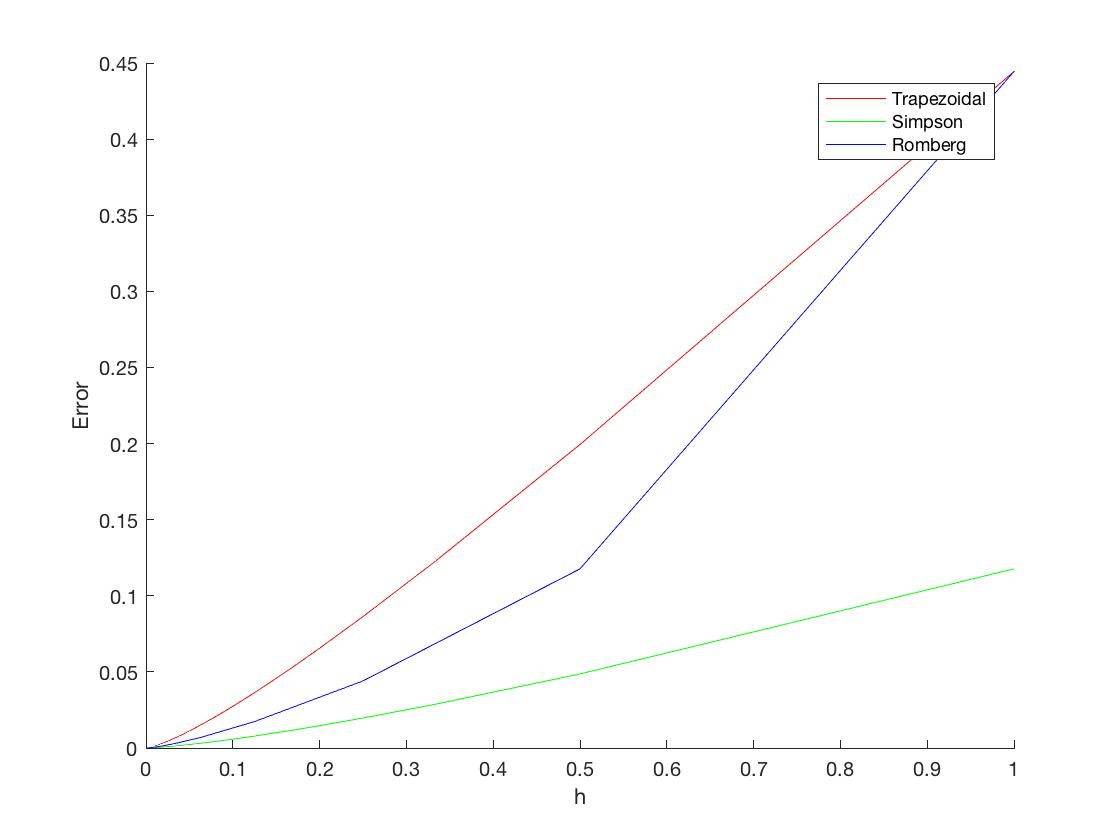
\includegraphics[width=15cm]{../image/H-Err.jpg}
    \caption{步长与误差图}
  \end{figure}
  \lstinputlisting{../src/draw.m}


\subsection{编写复化梯形公式的函数文件,命名为Trapezoidal.m,画出最大模误差与步长$h$的函数图像}
  \lstinputlisting{../src/Trapezoidal.m}

\subsection{编写复化Simpson公式的函数文件,命名为Simpson.m,画出最大模误差与步长$h$的函数图像}
  \lstinputlisting{../src/Simpson.m}

\subsection{比较两个公式的精度,回答问题:是否存在一个最小的$h$,使得精度不能再被改善?}
  复合梯形公式的误差为$O(h^2)$,复合Simpson公式的误差为$O(h^4)$. 从图中可知当$h<1$时,
  复合Simpson误差始终比复合梯形公式误差要小. 不存在一个最小的$h$,使得精度不能再提高.

\section{Romberg求积方法}
\subsection{编写Romberg公式的函数文件,命名为Romberg.m,画出最大模误差与步长$h$的函数图像}
  \lstinputlisting{../src/Romberg.m}

\newpage
\section{自适应Simpson求积方法}

\subsection{说明如何处理二分过程中树状图扩展的问题}
  \ilc{points}表示当前的各个区间的端点. 调用\ilc{separateInterval(l, r)}
  来递归划分区间$[l, r]$,如果在该区间上满足停机条件,则直接返回. 否则记
  $m = (l+r)/2$,递归划分区间$[l, m]$和$[m, r]$. 同时把新产生的点$m$加入
  \ilc{points}中. 最后将\ilc{points}升序排序即可. 

\subsection{编写自适应的程序,停止准则为精度达到$10^{-4}$,程序命名为AdaptSimpson.m}
  \lstinputlisting{../src/AdaptSimpson.m}
  对应各层划分出的区间为
  \begin{enumerate}
    \item $[0, 1]$
    \item $[0, 0.5]$,$[0,5, 1]$
    \item $[0, 0.25]$,$[0.25, 0.5]$
    \item $[0, 0.125]$,$[0.125, 0.25]$
    \item $[0, 0.0625]$,$[0.0625, 0.125]$
    \item $[0, 0.0312]$,$0.0312, 0.0625]$
    \item $[0, 0.0156]$,$[0.0156, 0.0312]$
    \item $[0, 0.00781]$,$[0.00781, 0.0156]$
    \item $[0, 0.00391]$,$[0.00391, 0.00781]$
    \item $[0, 0.00195]$,$[0.00195, 0.00391]$
    \item $[0, 0.000977]$,$[0.000977, 0.00195]$
    \item $[0, 0.000489]$,$[0.000489, 0.000977]$
    \item $[0, 0.000244]$,$[0.000244, 0.000489]$
    \item $[0, 0.000122]$,$[0.000122, 0.000244]$
    \item $[0, 0.0000610]$,$[0.0000610, 0.000122]$
    \item $[0, 0.0000305]$,$[0.0000305, 0.0000610]$
  \end{enumerate}








\end{document}
